%%%%%%%%%%%%%%%%%%%%%%%%%%%%%%%%%%%%%%%%%%%%%%%%%%%%%%%%%%%%%%%%%%%%%
% EPJ Web of Conferences -- proceedings draft
%
% DRAFT v3 -- trimmed for the 8-page limit.
% Items marked  %% TODO  need a decision or data before submission.
%%%%%%%%%%%%%%%%%%%%%%%%%%%%%%%%%%%%%%%%%%%%%%%%%%%%%%%%%%%%%%%%%%%%%
%
\documentclass{webofc}
\usepackage[varg]{txfonts}   % Web of Conferences font
\usepackage{tikz}
%
\begin{document}
%
\title{Binding DRBD promotion to containerised services:
       generating verified Pacemaker configurations for
       minimally-staffed scientific computing sites}
%
\author{\firstname{Geonmo} \lastname{Ryu}\inst{1}\fnsep\thanks{\email{geonmo@kisti.re.kr}}}

\institute{Korea Institute of Science and Technology Information (KISTI),
           Daejeon, Republic of Korea}

\abstract{%
  Small scientific computing sites run a handful of stateful grid
  services on a handful of machines, administered by one or two people
  for whom cluster operation is one duty among several. Such sites need
  real high availability but cannot absorb the operational surface of a
  general-purpose orchestrator. Our design follows from three
  constraints: a small team argues for the availability layer the
  operating-system vendor supports directly, so we use Pacemaker and
  Corosync rather than a separate control plane; containerised services
  argue for Podman Quadlet, which turns container definitions into
  ordinary systemd units that Pacemaker manages without an adapter; and
  the absence of external shared storage -- no NFS server, no SAN --
  makes DRBD replication between the cluster nodes the means by which a
  service finds its configuration and state on whichever node currently
  runs it. The hard part of this stack is the chain of Pacemaker
  resource, operation and constraint definitions that binds DRBD
  promotion to the start of the dependent containers, because its
  failure modes are silent: several configurations are accepted by every
  tool and are nevertheless wrong. We describe that chain in detail, and
  the tool we built to generate it -- \emph{IPVLAN Container Manager},
  which emits DRBD resource files, Quadlet units, \texttt{pcs} setup and
  teardown scripts, nftables ingress policy and the deploying Ansible
  playbooks, while adding no runtime component to the cluster. We report
  the validation strategy adopted after unit tests were found to accept
  artefacts that the real tools reject, and experience from the
  production three-node deployment of the CMS Tier-2 site
  T2\_KR\_KISTI.
}
%
\maketitle
%
%%%%%%%%%%%%%%%%%%%%%%%%%%%%%%%%%%%%%%%%%%%%%%%%%%%%%%%%%%%%%%%%%%%%%
\section{Introduction}
\label{sec:intro}

High availability is usually a question of scale, but many scientific
computing sites are constrained instead by the number of people
available to operate the system: a CMS Tier-2/3 site typically runs a
handful of services that must not be down for long -- a storage
front-end, a compute-element gateway, an accounting
publisher -- on three to seven machines, administered by one or two
staff with other duties. For that population, an HA deployment's
dominant cost is not hardware but the operational knowledge a small team
must keep resident and recoverable after weeks-long interruptions: a
control plane that is itself a distributed system to keep alive, upgrade
and debug (as in Kubernetes~\cite{kubernetes}) trades one operational
problem for a larger one, while managing containers by hand is
error-prone and has no central place for the availability logic to
live.

\subsection{Three constraints and the choices they force}
\label{sec:choices}

\paragraph{A small team implies a vendor-supported availability layer.}
When the operating team is small, a component's most valuable property
is not its feature set but the existence of someone else's
documentation, errata and support contract. On RHEL~9 and its
derivatives that component is Pacemaker with
Corosync~\cite{pacemaker,corosync,rhelha}: vendor-documented, with
failure modes described in material an administrator can reach without
reading source code. Maturity is what a site with no platform team
should be buying, so we build on Pacemaker rather than a second control
plane.

\paragraph{Containerised services imply a runtime that systemd -- and
therefore Pacemaker -- already understands.}
These sites increasingly distribute their services as containers, so the
availability layer must manage containers, not packages. Podman with
Quadlet resolves this without an adapter~\cite{podman,quadlet}: Quadlet
turns declarative unit files into systemd services at generator time,
and Pacemaker manages systemd units natively -- no container-specific
resource agent, daemon or second lifecycle manager required.

\paragraph{No external shared storage implies replication between the
nodes themselves.}
A classical Pacemaker service assumes the failing-over data is reachable
from every node, typically an NFS server or a SAN -- infrastructure our
target sites lack, and adding it would just create a new single point of
failure. What these services carry across a failover is not bulk data
but a small, write-sensitive working set: a configuration tree, a job
spool, cached accounting records. DRBD~\cite{drbd9} replicates that
synchronously between the nodes and exposes a single virtual block
device, so the service finds an identical configuration and state
directory wherever it currently runs, with no storage appliance
involved.

A fourth characteristic shapes networking rather than availability.
Data-intensive workloads are sensitive to container-networking overhead:
a bridge-and-NAT path or VXLAN overlay adds per-packet work and an
address space invisible outside the host. The in-kernel IPVLAN
driver~\cite{ipvlan} in L2 mode instead attaches a container directly to
a physical NIC with an address on the physical subnet -- an ordinary LAN
host to clients, firewalls and monitoring alike, keeping that address
across a restart on another node.

\subsection{The remaining problem, and our contribution}

Each of these four components is individually well documented; the
difficulty is the \emph{seams} between them -- a working three-node
service needs a DRBD resource file, an LVM layout, a Quadlet unit set, a
promotable clone with ordering and colocation constraints in the correct
role and direction, a fencing device, and a firewall policy identical on
every node, and keeping all of it mutually consistent after a change is
exactly the work that does not survive being interrupted.

Our contributions are: a detailed account of the DRBD-to-Pacemaker
promotion chain and the ways plausible-looking definitions fail silently
(Sect.~\ref{sec:promote}); a generator-based tool that emits that chain
with the rest of the stack, under the policy that every cluster-state
change is a generated Ansible playbook rather than a direct command
(Sect.~\ref{sec:design}); a validation strategy checking generated
artefacts against the real deployment tools with negative controls, and
the defects this uncovered that substring unit tests had accepted
(Sect.~\ref{sec:validation}); and experience from the production
deployment at CMS Tier-2 site T2\_KR\_KISTI (Sect.~\ref{sec:deployment}).

%%%%%%%%%%%%%%%%%%%%%%%%%%%%%%%%%%%%%%%%%%%%%%%%%%%%%%%%%%%%%%%%%%%%%
\section{The DRBD--Pacemaker promotion chain}
\label{sec:promote}

\subsection{What promotion has to guarantee}

For a containerised service whose configuration and state live on a
replicated device, a correct failover must satisfy four properties at
once:

\begin{enumerate}
\item \textbf{Exclusivity.} At most one node holds the DRBD device in
      the primary role at any time. Two primaries with a mounted
      non-cluster filesystem means divergent state.
\item \textbf{Ordering.} The filesystem is mounted only after promotion
      completes, and the containers start only after the mount succeeds.
      On relocation the reverse must hold: containers stop, filesystem
      unmounts, device demotes.
\item \textbf{Co-location.} The mount and the containers run on the node
      holding the promoted instance, not merely on \emph{some} node.
\item \textbf{Observability of failure.} If promotion fails or the
      promoted instance becomes unhealthy, the cluster must take a
      defined action, and that action must be the one the administrator
      configured.
\end{enumerate}

Properties 1--3 are expressed with resource and constraint definitions;
property 4 depends on an interaction between the resource's
\texttt{on-fail} setting and cluster-wide fencing configuration, and is
the least obvious of the four.

\subsection{Primitive and promotable clone}

DRBD is registered with the LINBIT-provided OCF agent and then converted
into a promotable clone, as in Listing~\ref{lst:drbd}.

\begin{figure}[h]
\begin{scriptsize}
\begin{verbatim}
pcs resource create drbd-r0 ocf:linbit:drbd \
    drbd_resource=r0 \
    op demote  interval=0s  timeout=90s \
    op monitor interval=29s role=Promoted \
               on-fail=fence \
    op monitor interval=31s role=Unpromoted \
    op notify  interval=0s  timeout=90s \
    op promote interval=0s  timeout=90s \
    op reload  interval=0s  timeout=30s \
    op start   interval=0s  timeout=240s \
    op stop    interval=0s  timeout=100s
pcs resource promotable drbd-r0 \
    promoted-max=1 promoted-node-max=1 \
    clone-max=3 clone-node-max=1 \
    notify=true id=drbd-r0-clone
\end{verbatim}
\end{scriptsize}
\caption{Generated DRBD promotable clone definition. The full operation
set is emitted explicitly rather than left to agent defaults, and the
two role-scoped monitors carry deliberately different intervals; see
Sect.~\ref{sec:monitor}.}
\label{lst:drbd}
\end{figure}

\texttt{promoted-max=1} with \texttt{promoted-node-max=1} enforces
exclusivity (property~1), and \texttt{notify=true} is required by the
DRBD agent, which uses clone notifications to coordinate role changes
among peers. The operation set is written out in full because the
agent's defaults differ from the values the DRBD documentation
recommends for a Pacemaker-managed resource, and a partially specified
set is indistinguishable, on inspection of the CIB, from a deliberately
chosen one.

\subsection{Role-scoped monitors and the interval collision}
\label{sec:monitor}

A promotable DRBD clone needs two recurring monitors, one per role,
because the health criteria differ: a promoted instance must be primary
and connected, an unpromoted instance must be secondary and in sync. The
obvious encoding is two monitors with the same interval and different
\texttt{role} attributes.

That encoding is rejected: \texttt{pcs} (observed with version 0.11.11)
refuses the resource creation, because the operation identity it
constructs does not include the role, so two monitors at the same
interval collide regardless of role. The tool therefore emits distinct
intervals and, following LINBIT's own examples, chooses values that are
not multiples of one another (\texttt{29s} and \texttt{31s} by default)
so the two monitors do not repeatedly coincide. A regression test
asserts both that two role-scoped monitors are present and that their
default intervals are mutually non-divisible.

The placement of \texttt{on-fail} is a related subtlety. It is attached
to the \emph{promoted}-role monitor only, because the set of values the
interface offers (\texttt{fence}, \texttt{block}, \texttt{stop},
\texttt{ignore}, \texttt{demote}) is fully valid only there: Pacemaker
accepts \texttt{demote} only for the \texttt{promote} action and for
recurring monitors with \texttt{role=Promoted}. Attaching the same value
to the unpromoted monitor produces a definition that \texttt{pcs}
rejects for some user choices and accepts for others -- input-dependent
breakage, which is unpleasant to diagnose in the field.

\subsection{The ordering and colocation chain}

With the clone defined, the dependent resources are chained. For a
service with one DRBD volume, a filesystem and a container group, the
tool generates:

\begin{scriptsize}
\begin{verbatim}
pcs constraint order promote drbd-r0-clone \
    then start fs-r0 kind=Mandatory \
    id=ord-fs-r0-after-drbd-r0-clone
pcs constraint colocation add fs-r0 \
    with Promoted drbd-r0-clone \
    score=INFINITY \
    id=col-fs-r0-with-drbd-r0-clone
pcs constraint order start fs-r0 \
    then start grp-myapp kind=Mandatory \
    id=ord-grp-myapp-after-fs-r0
pcs constraint colocation add grp-myapp \
    with fs-r0 score=INFINITY \
    id=col-grp-myapp-with-fs-r0
\end{verbatim}
\end{scriptsize}

The ordering constraints give property~2 and the colocation constraints
property~3; Pacemaker derives the reverse order on relocation
automatically. Two details were wrong in earlier versions. First, the
role qualifier in \texttt{pcs constraint colocation add} belongs
\emph{before} the resource identifier (\texttt{... with Promoted
drbd-r0-clone}), not appended as an option -- syntactically valid but
schema-invalid, and, unguarded, a silently absent constraint
(Table~\ref{tab:defects}). Second, constraints on a pod-plus-containers
service must attach to the group, not its members: an unnormalised empty
\texttt{after\_fs} value used to make the generator's filter match
neither the "has a filesystem" nor the "has none" branch, emitting
colocation against each member individually and defeating the group --
now normalised in the route handler, with a test asserting constraints
never name a member directly.

A related pitfall: \texttt{clone-max} bounds how many clone instances
Pacemaker instantiates, and a value hardcoded below the cluster's actual
node count silently excludes the remaining nodes from ever holding a
DRBD instance -- valid configuration, available service, and those nodes
simply never failover candidates. The tool now derives \texttt{clone-max}
from the selected node count instead of a fixed default.

\subsection{Fencing: two switches that must agree}

Property~4 depends on two independent settings that are easy to
configure inconsistently.

The first is the resource-level \texttt{on-fail} attribute: if
\texttt{on-fail=fence} is set while \texttt{stonith-enabled=false},
\texttt{pcs} accepts the configuration, but Pacemaker silently downgrades
the action to \texttt{stop} at runtime -- fencing was selected, no error
is reported, and none occurs. Because this combination is realistic
(fencing is often disabled while a test cluster is built), the generator
detects it and emits an explicit warning naming the affected resources.
STONITH itself is configured as one \texttt{fence\_ipmilan} device per
node, which is what actually prevents the split-brain scenario
property~1 rules out at the resource level.

The second is DRBD's own fencing policy. \texttt{fencing resource-only}
instructs DRBD to consult the cluster before promoting, through a
\emph{fence-peer handler}; without it, a promotion attempted while the
peer is unreachable does not fail quickly, but blocks until the
Pacemaker operation timeout expires and is then reported as a failure.
The generator therefore deploys \texttt{crm-fence-peer.9.sh} in
\texttt{/etc/drbd.d/global\_common.conf} whenever \texttt{resource-only}
fencing is selected, stating the dependency where the policy is chosen.

\subsection{Multiple volumes: colocation has a direction}

A service depending on more than one DRBD volume needs them promoted on
the same node, via a directed colocation between two promotable clones --
one anchors, the other follows, as \texttt{Promoted follower with
Promoted anchor}. Generating this backwards is accepted but blocks
relocation of the follower alone with an unexplained \texttt{-INFINITY}
score, so the interface presents an explicit anchor/follower pair and
labels which side to move.

\subsection{Idempotency and teardown}

Two properties proved necessary once the tool ran against an
already-existing cluster. First, \emph{idempotency}: since the script
runs under \texttt{set -euo pipefail}, a \texttt{pcs resource create}
failing with "already exists" stops the run there, leaving a partially
configured cluster and an administrator who must work out by hand how
far it got. Every resource and constraint creation is now wrapped in an
existence check, so re-running on a configured cluster is a no-op that
reports what it skipped.

Second, \emph{teardown}: a generator that can only create is of little
use once a configuration must be revised, since the administrator must
inspect the CIB and decide what to delete -- exactly the task the tool
exists to remove. The tool emits a matching teardown script that removes
only what it created, in reverse dependency order (constraints, groups,
systemd and filesystem resources, the DRBD clone, then STONITH), since a
remaining constraint blocks resource deletion and a remaining group
blocks member deletion. Resources are stopped normally, not with
\texttt{--force}, so the filesystem unmounts and DRBD demotes cleanly;
the script never touches the DRBD volume or the \texttt{.res} file,
withdrawing the storage from Pacemaker management while leaving the data
alone. Tests assert the ordering, re-runnability, and the absence of any
storage-destroying command.

%%%%%%%%%%%%%%%%%%%%%%%%%%%%%%%%%%%%%%%%%%%%%%%%%%%%%%%%%%%%%%%%%%%%%
\section{Generating the stack}
\label{sec:design}

\subsection{A generator, not a controller}

The chain of Sect.~\ref{sec:promote} is what \emph{IPVLAN Container
Manager} produces. The central design decision is that the tool produces
text and gets out of the way: no agent on the cluster nodes, no
reconciliation loop, no runtime dependency on the tool being available.
A generator can be abandoned without stranding the cluster, whereas a
controller cannot -- and if the site later manages the cluster by hand,
the artefacts produced are exactly what a handwritten deployment would
contain. This is the reasoning of Sect.~\ref{sec:choices} again: minimise
the components whose continued existence the site depends on. Every
artefact is a complete file with comments stating \emph{why} a setting is
present; for a two-person team, a script whose comments record that
\texttt{on-fail=fence} is inert while \texttt{stonith-enabled=false} is
worth more than a graphical rendering of the same configuration.

The application is a single Rust binary with no server-side session
state; each submission independently transforms a set of values into the
files of Table~\ref{tab:artefacts}, and a small SQLite database holds
only inventory that must persist across restarts. A background task
scans existing DRBD, Quadlet and \texttt{pcsd} state at startup, so an
administrator with a partially configured cluster does not start from an
empty form. Each generator is a pure function from a model structure to
a string -- what makes the validation strategy of
Sect.~\ref{sec:validation} possible.

\begin{table}
\centering
\caption{Artefacts generated from the web interface. Each row
corresponds to one pure generator function and one set of tests.}
\label{tab:artefacts}
\begin{tabular}{lll}
\hline
Subsystem & Artefact & Consumer \\\hline
DRBD           & \texttt{<res>.res} + playbook        & \texttt{drbdadm} \\
Quadlet        & \texttt{.container}, \texttt{.pod},  & \texttt{podman} \\
               & \texttt{.network}, \texttt{.volume}  & (quadlet generator) \\
Pacemaker      & \texttt{pcs} setup script,           & \texttt{pcs} \\
               & teardown script, playbook            & \\
Firewall       & \texttt{table netdev} policy         & \texttt{nft} \\\hline
\end{tabular}
\end{table}

\subsection{Ansible as the only mutation path}

Early in development the tool could execute a few commands directly on
cluster nodes, e.g.\ to inspect firewall state while diagnosing a
failover. This was removed: any change to a cluster node's state must
now be expressed as a generated Ansible playbook~\cite{ansible} the
administrator can read before running and re-run afterwards.

The reason is not purity: a direct command is invisible afterward -- it
appears in no artefact, cannot be reviewed, and cannot be replayed on a
node that was down at the time. At a minimally-staffed site that last
property matters most, since the person applying a change is often not
the one diagnosing its consequence weeks later. Two facilities follow: a
playbook that runs \texttt{ip -j addr show} on every node to discover
which interface carries a given subnet, and, when a network's parent
interface is still unknown at generation time, a placeholder
(\texttt{Options=parent=\_\_PARENT\_IFACE\_\_}) that a deployment-time
detection task replaces, so the generated unit is correct despite
differing interface names.

%%%%%%%%%%%%%%%%%%%%%%%%%%%%%%%%%%%%%%%%%%%%%%%%%%%%%%%%%%%%%%%%%%%%%
\section{Validating generated artefacts}
\label{sec:validation}

The natural way to test a generator is to assert its output contains the
expected substrings. We did this, and the tests passed while the
generated artefacts were rejected by the tools that consume them: a
substring assertion encodes the same intent as the generator, written by
the same author at the same time, so if that intent is wrong -- e.g.\
believing \texttt{on-io-error passthrough} is a valid DRBD option --
generator and test simply agree.

We therefore added a permanent test module that submits generated
artefacts to the real tools -- \texttt{drbdadm}, \texttt{nft --check},
the Podman Quadlet generator, and \texttt{ansible-playbook
--syntax-check} with \texttt{ansible-inventory --graph} -- each skipped
with a reported reason when its binary is absent, and each paired with a
\emph{negative control}: a deliberately invalid artefact the validator
must reject, so a validator silently reduced to a no-op cannot be
mistaken for a passing one. This caught exactly that situation once
during development.

Table~\ref{tab:defects} lists the defects this uncovered that the
substring tests had accepted -- most semantic, and four of seven that
would have manifested only during a failover. One is worth singling out:
two nftables sets with colliding names are not rejected by \texttt{nft}
but silently \emph{merged}, granting more access than specified -- a
firewall that fails open. The suite currently contains 79 tests,
including the external validations.

\begin{table}
\centering
\caption{Defects in generated artefacts found by external-tool
validation, none of which had been detected by substring assertions.}
\label{tab:defects}
\begin{footnotesize}
\begin{tabular}{p{0.44\textwidth}p{0.19\textwidth}p{0.25\textwidth}}
\hline
Defect & Found by & Consequence \\\hline
Jinja \texttt{search()} pattern with an unescaped literal
\texttt{(} & Python \texttt{re} & playbook aborts \\
\texttt{hosts:} value containing a newline & YAML parser & play targets wrong hosts \\
\texttt{on-io-error passthrough} is not a valid DRBD~9
value, and was the generator default & \texttt{drbdadm} & resource file rejected \\
\texttt{after-sb-1pri call-pri-lost} is not a valid value & \texttt{drbdadm} & resource file rejected \\
Two role-scoped monitors with identical intervals & real cluster & whole script aborts \\
Colocation role qualifier in the option position & real cluster & constraint absent; mount fails on failover \\
Singleton configuration tables accumulating duplicate rows & explicit test & configuration read is non-deterministic \\\hline
\end{tabular}
\end{footnotesize}
\end{table}

%%%%%%%%%%%%%%%%%%%%%%%%%%%%%%%%%%%%%%%%%%%%%%%%%%%%%%%%%%%%%%%%%%%%%
\section{Production deployment}
\label{sec:deployment}

The stack is in production on a three-node AlmaLinux~9 cluster at
T2\_KR\_KISTI, the CMS Tier-2 site operated by KISTI, managing the
dCache~\cite{dcache} frontend, HTCondor-CE~\cite{htcondorce,condor} and
site-BDII/APEL~\cite{apel} information and accounting services. All
three match the design's target profile: single-instance, stateful
services whose unavailability is immediately visible to the
collaboration, each needing a modest configuration and state directory
rather than bulk storage -- the working set DRBD replication is suited
to, and the reason no NFS or SAN layer is involved. Each service is a
Quadlet-defined container group registered with Pacemaker as a systemd
resource, colocated with the filesystem resource carrying its
configuration, in turn colocated with the promoted DRBD instance,
following the chain of Sect.~\ref{sec:promote}. IPVLAN L2 networks attach
the containers directly to the nodes' physical interfaces, so each
service keeps a stable, routable address across a failover
(Fig.~\ref{fig:arch}). All deployment uses the generated playbooks; no
configuration change is applied to a node by hand.

\begin{figure}[h]
\centering
\resizebox{0.62\linewidth}{!}{%
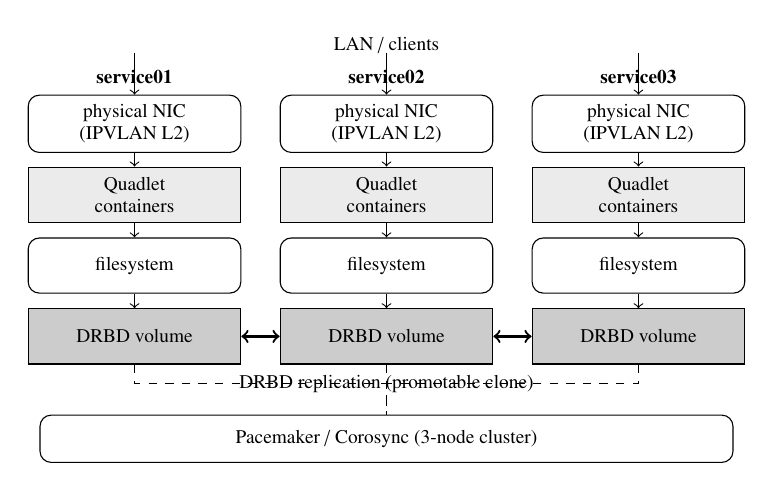
\begin{tikzpicture}[
  font=\scriptsize,
  every node/.style={align=center},
  box/.style={draw, rounded corners, minimum width=27mm, minimum height=7mm},
  svcbox/.style={draw, fill=black!8, minimum width=27mm, minimum height=7mm},
  drbdbox/.style={draw, fill=black!20, minimum width=27mm, minimum height=7mm},
]
\def\dx{32mm}
\foreach \i/\name in {1/service01, 2/service02, 3/service03} {
  \node[font=\bfseries\scriptsize] (lbl\i) at (\i*\dx, 30mm) {\name};
  \node[box] (nic\i) at (\i*\dx, 24mm) {physical NIC\\(IPVLAN L2)};
  \node[svcbox] (ctr\i) at (\i*\dx, 15mm) {Quadlet\\containers};
  \node[box] (fs\i) at (\i*\dx, 6mm) {filesystem};
  \node[drbdbox] (drbd\i) at (\i*\dx, -3mm) {DRBD volume};
  \draw[->] (\i*\dx, 33mm) -- (nic\i);
  \draw[->] (nic\i) -- (ctr\i);
  \draw[->] (ctr\i) -- (fs\i);
  \draw[->] (fs\i) -- (drbd\i);
  \draw[dashed] (drbd\i) -- ++(0,-6mm) -| (2*\dx,-13mm);
}
\node[align=center] at (2*\dx, 34mm) {LAN / clients};
\draw[<->, thick] (drbd1) -- (drbd2);
\draw[<->, thick] (drbd2) -- (drbd3);
\node at (2*\dx, -9mm) {DRBD replication (promotable clone)};
\node[box, minimum width=88mm, minimum height=6mm] (pcmk) at (2*\dx, -16mm) {Pacemaker / Corosync (3-node cluster)};
\end{tikzpicture}%
}
\caption{The three-node production deployment: on each node, IPVLAN L2
attachment to the physical interface, a Quadlet container group (dCache
frontend, HTCondor-CE or site-BDII/APEL), and a filesystem resource
colocated with the promoted DRBD instance; DRBD replicates configuration
and state between the nodes, and Pacemaker/Corosync own promotion and
placement across all three.}
\label{fig:arch}
\end{figure}

Because the tool only ever adds, drift between what it can generate and
what is actually running had accumulated in the primitives themselves.
Five of the six deployed DRBD resources (\texttt{cecm\_config},
\texttt{drbd\_bdii}, \texttt{drbd\_mariadb}, \texttt{drbd\_db},
\texttt{drbd\_dcache}) still carried a single, non-role-scoped monitor at
a flat 20\,s, predating the refinement of Sect.~\ref{sec:monitor}, and
the sixth (\texttt{drbd\_cecm\_varlib}) paired a 10\,s promoted-role
monitor with a 20\,s unpromoted-role one -- an exact multiple, the
pattern that refinement exists to avoid; none set \texttt{on-fail=fence}.
We corrected this directly on the live cluster: each primitive now
carries role-scoped monitors with non-divisible intervals (17\,s/19\,s,
or 10\,s/19\,s for \texttt{drbd\_cecm\_varlib}) and
\texttt{on-fail=fence} on the promoted-role monitor only, leaving
promote, demote and filesystem-start operations untouched so a transient
failure during relocation still gets a retry rather than an immediate
fence. The change was staged offline, schema-validated and diffed
against the running configuration before being pushed; no resource
stopped, restarted or relocated, and no failcount appeared afterward. It
was applied by hand with \texttt{pcs}, not through the generated
playbook of Sect.~\ref{sec:design}, because the tool has no mechanism to
reconcile an already-running resource's operation set with its current
defaults -- the drift-detection gap Sect.~\ref{sec:discussion} lists as a
limitation, closed here by hand rather than by the tool itself.

Relocation of a DRBD-backed service between nodes completes in the
expected sequence: containers stopped, filesystem unmounted, DRBD
demoted on the source, promoted on the target, filesystem mounted,
containers started. The constraint chain of Sect.~\ref{sec:promote} was
necessary and sufficient for this, and the failures described there were
all encountered on the way to it.

We can quantify this from \texttt{pacemaker.log} on service01, retained
without gaps since 2026-02-12. Before the fence-peer handler was deployed
(Sect.~\ref{sec:promote}, commit \texttt{df0c377}, applied 2026-07-23
17:06 KST), every relocation recorded in that window failed outright:
with the peer unreachable, promotion blocked for the full operation
timeout (90\,s for demote, 120\,s for promote) and was then reported as a
resource failure rather than completing -- the failure mode described in
Sect.~\ref{sec:promote}. After the fix, four administrator-triggered
relocations (\texttt{pcs resource move}) of the production services
completed as shown in Table~\ref{tab:failover}: HTCondor-CE (2 DRBD
volumes, 2 filesystems, 1 systemd resource) service01$\to$service02 in
7.8\,s; site-BDII/APEL, whose accounting-database volume follows the
site-BDII volume under the multi-volume colocation of
Sect.~\ref{sec:promote} (2 DRBD volumes, 2 filesystems, 4 systemd
resources) service03$\to$service01 in 6.9\,s and, in the reverse
direction three days later, in 6.8\,s; and dCache (2 DRBD volumes, 2
filesystems, 13 systemd-managed containers) service03$\to$service01 in
1\,min\,55\,s, excluding an external monitoring gate unrelated to
Pacemaker. DRBD promotion itself completed in the same single-digit-second
range in all four cases; dCache's outlier duration is accounted for by
its thirteen containers starting in the sequence the group resource
imposes, not by a slower promotion or filesystem check. The handler fix
therefore did not make relocation faster: it made it succeed. These
figures are for administrator-initiated moves rather than an unplanned
node loss; measuring the latter under the fixed configuration remains
future work (Sect.~\ref{sec:discussion}).

\begin{table}[h]
\centering
\caption{Resource composition and relocation time for
administrator-triggered moves of the production services, measured after
the fence-peer handler fix of Sect.~\ref{sec:promote}.}
\label{tab:failover}
\begin{tabular}{lccc}
\hline
Service & DRBD vols. & Resources & Relocation \\\hline
HTCondor-CE     & 2 & 5  & 7.8\,s \\
site-BDII/APEL  & 2 & 8  & 6.9\,s / 6.8\,s \\
dCache          & 2 & 17 & 1\,min\,55\,s \\\hline
\end{tabular}
\end{table}

Because IPVLAN places containers on the physical subnet, access control
cannot be delegated to a NAT boundary. The tool generates an nftables
\texttt{table netdev} ingress policy~\cite{nftables} with per-target
address sets, subnet groups and per-service port sets, installed
identically on \emph{every} node rather than only the one currently
running the service -- after a failover the destination is served
elsewhere, and a node without the rule drops the traffic. Enforcement is
kept at the host level rather than delegated to \texttt{firewalld}'s
per-service zones, since a Quadlet-managed container is not a service
firewalld itself starts or tracks, so whether one is actually running is
not something its zone/service rule model can determine reliably.

%%%%%%%%%%%%%%%%%%%%%%%%%%%%%%%%%%%%%%%%%%%%%%%%%%%%%%%%%%%%%%%%%%%%%
\section{Discussion and conclusion}
\label{sec:discussion}

We have described the chain of Pacemaker definitions binding DRBD
promotion to the start of containerised services, and the configurations
every tool accepts that are nevertheless wrong: monitor operations whose
role does not disambiguate their interval, a colocation role qualifier
in the option position, a clone count that silently excludes nodes, a
colocation between promotable clones generated backwards, and a fencing
action downgraded at runtime without notice. What these share is that
none is detected at configuration time, only at failover time -- the one
moment a minimally-staffed site has no capacity to debug. Encoding them
once, in a generator, is worth more than documenting them.

The most transferable result is arguably the testing discipline of
Sect.~\ref{sec:validation}. A configuration generator is a compiler
whose back end is someone else's parser; testing it against one's own
beliefs about that parser is not testing. The cost of running the real
validators in continuous integration was small; the cost of the defects
they found, had they reached a production failover, would not have been.

The design targets sites whose binding constraint is operator attention
rather than capacity: a handful of stateful services, three to seven
machines, one or two administrators with other duties, and no external
shared storage; a site needing elasticity, dynamic scheduling or
multi-tenancy is better served by a general-purpose orchestrator. One
limitation is worth stating: there is no drift detection -- because the
tool generates and leaves, a hand-changed configuration is not noticed
until the next scan, and the scan is informational rather than
corrective.

Finally, the choices of Sect.~\ref{sec:choices} were made with an
eventual migration in mind: because the services are packaged as OCI
containers and described declaratively, the unit of deployment is
already what a container orchestrator would schedule -- only the
availability and storage layer is specific to this stack, not the
workload definition. We consider that claim provisional until
demonstrated, and it -- together with failover measurements under an
actual unplanned node loss rather than the administrator-initiated
relocations of Sect.~\ref{sec:deployment}, quantitative networking
measurements, and divergence reporting between generated and live
configuration -- is the direction of future work.

%%%%%%%%%%%%%%%%%%%%%%%%%%%%%%%%%%%%%%%%%%%%%%%%%%%%%%%%%%%%%%%%%%%%%
\section*{Declaration on the use of generative AI}

During preparation of this manuscript the author used Claude Code
(Anthropic), an AI coding and writing assistant, across several Claude
model versions including Claude Sonnet 5, to assist with LaTeX
formatting, with editing prose for language and clarity, and with
organising the log- and \texttt{pcs}-derived measurements reported in
Sect.~\ref{sec:deployment} from data the author supplied. All
AI-assisted content, including the measurements and their sourcing, was
reviewed and verified by the author, who takes full responsibility for
the content of this publication. The tool is not an author and is not
cited as a source.

%%%%%%%%%%%%%%%%%%%%%%%%%%%%%%%%%%%%%%%%%%%%%%%%%%%%%%%%%%%%%%%%%%%%%
\begin{thebibliography}{99}

\bibitem{kubernetes}
Kubernetes documentation, The Kubernetes Authors,
\texttt{kubernetes.io/docs}

\bibitem{pacemaker}
\textit{Pacemaker Explained}, ClusterLabs,
\texttt{clusterlabs.org/pacemaker/doc}

\bibitem{corosync}
Corosync Cluster Engine documentation, ClusterLabs,
\texttt{corosync.github.io/corosync}

\bibitem{rhelha}
\textit{Configuring and managing high availability clusters},
Red Hat Enterprise Linux 9 documentation, Red Hat,
\texttt{docs.redhat.com}

\bibitem{podman}
Podman documentation, Containers project,
\texttt{docs.podman.io}

\bibitem{quadlet}
\texttt{podman-systemd.unit} (Quadlet) manual page, Containers project,
\texttt{docs.podman.io/en/latest/markdown/podman-systemd.unit.5.html}

\bibitem{drbd9}
\textit{The DRBD 9 User's Guide}, LINBIT,
\texttt{linbit.com/drbd-user-guide}

\bibitem{ipvlan}
IPVLAN driver HOWTO, Linux kernel documentation,
\texttt{docs.kernel.org/networking/ipvlan.html}

\bibitem{nftables}
nftables wiki, Netfilter project,
\texttt{wiki.nftables.org}

\bibitem{ansible}
Ansible documentation, Red Hat,
\texttt{docs.ansible.com}

\bibitem{dcache}
P.~Fuhrmann, V.~G\"ulzow, \textit{dCache, Storage System for the
Future}, in Euro-Par 2006 Parallel Processing, Lecture Notes in Computer
Science \textbf{4128} (Springer, Berlin, 2006) pp.~1106--1113

\bibitem{htcondorce}
HTCondor-CE documentation, HTCondor Software Suite, University of
Wisconsin--Madison, \texttt{htcondor.com/htcondor-ce}

\bibitem{condor}
D.~Thain, T.~Tannenbaum, M.~Livny, Concurrency and Computation: Practice
and Experience \textbf{17}, 323--356 (2005)

\bibitem{apel}
M.~Jiang, C.~Del Cano Novales, G.~Mathieu, J.~Casson, W.~Rogers,
J.~Gordon, \textit{An APEL Tool Based CPU Usage Accounting
Infrastructure for Large Scale Computing Grids}, in Data Driven
e-Science (Springer, New York, 2011) pp.~175--186

\end{thebibliography}

\end{document}
